\documentclass[12pt]{article}
\usepackage[a4paper,margin=1in]{geometry}
\usepackage[T1]{fontenc}
\usepackage[utf8]{inputenc}
\usepackage{graphicx}
\usepackage{booktabs}
\usepackage{multirow}
\usepackage{array}
\usepackage{setspace}
\usepackage{float}
\usepackage{amsmath}
\usepackage{xcolor}

\title{\textbf{Mirror Reflection Agent: A Reliability-Control Architecture for Bounded Scientific Reasoning}}
\author{Brook \\ Independent Researcher}
\date{}

\begin{document}
\maketitle
\onehalfspacing
\emergencystretch=2em

\begin{abstract}
Large language models are increasingly used in scientific workflows, but their usefulness is often limited by unsupported certainty, loss of source conditions, and weak retention of prior corrections. This paper presents Mirror Reflection Agent, a reliability-control architecture that externalizes candidate cognition as a \texttt{MindState}, critiques it through typed \texttt{MirrorVerdict} actions, and stores correction-lineage memory for later reuse. The current implementation is evaluated with a deterministic three-track benchmark that avoids LLM-as-judge scoring and spans 86 cases and 318 executed runs across ablation, science-facing question answering, and longitudinal correction retention. In the ablation benchmark, pass rate rises from 0.17 in the direct-answer baseline to 0.57 with mirror control and 0.70 with memory-backed reflective modes, while condition preservation rises from 0.00 to 0.60 and correction retention rises from 0.00 to 0.13. In the science-facing benchmark, reflective modes raise pass rate from 0.00 to 0.92 on constants-and-units questions and from 0.00 to 1.00 on abstention-boundary cases, while condition-sensitive property cases remain limited to 0.33 pass despite improved condition preservation. In the longitudinal benchmark, cross-session correction retention reaches 0.60 in the dual-memory configuration versus 0.00 for the direct baseline, while memory-scope isolation remains at 0.20 and recurrence remains unresolved for one sequence family. These results support Mirror Reflection Agent as an auditable mechanism for improving bounded scientific reasoning behavior within the current benchmark.
\end{abstract}

\noindent\textbf{Keywords:} reflective agents, reliability control, bounded scientific reasoning, memory, uncertainty, AI for science

\section{Introduction}

Scientific uses of language models demand more than fluent text generation. In scientific settings, a useful system must preserve source conditions, separate structured evidence from weak prior knowledge, express uncertainty when evidence is incomplete, and retain prior corrections without collapsing back into stale templates. These requirements are stricter than those of general-purpose question answering because a numerically plausible answer can still be misleading if its units, assumptions, or operating conditions are not made explicit. Recent work on chain-of-thought prompting and acting-reasoning loops has improved complex inference, but these methods do not by themselves guarantee auditable control over factual boundaries or condition-sensitive claims \cite{cot,react,toolformer}.

Existing reflective pipelines improve generation through refinement, retrieval, or tool use \cite{selfrefine,reflexion,critic,selfrag}. However, several reliability gaps remain unresolved. Intermediate reasoning is often hidden inside free-form text instead of being represented as an inspectable state object. Critique is frequently expressed as style advice rather than as an explicit control decision that can revise, retrieve, wait, or diverge. Correction history is also commonly stored as unstructured text, which makes it difficult to reuse prior lessons as stable lineage across later tasks. These limitations are especially consequential in scientific use because condition loss, overclaiming, and weak correction reuse can all produce outputs that look plausible while remaining operationally unreliable.

The present architecture is designed around those gaps. Mirror Reflection Agent externalizes candidate reasoning as a structured \texttt{MindState}, critiques it through typed \texttt{MirrorVerdict} actions, and stores correction-lineage memory together with reusable strategy traces. To evaluate this design, the paper introduces a deterministic three-track benchmark covering ablation, science-facing question answering, and longitudinal correction reuse, and reports evidence from 86 cases and 318 executed runs. The resulting contribution is a systems and mechanism study of bounded scientific reasoning behavior: it aims to show what explicit state, typed critique, and memory can already improve within the current benchmark, without extending that claim to broad scientific superiority.

This focus differs from recent self-reflection systems designed to improve academic response writing or other general language-generation tasks \cite{academicresponse}. In those settings, reflection primarily helps the model produce more relevant and persuasive text. The present paper targets a different failure surface: whether a system can preserve scientific conditions, avoid unsupported factual extrapolation, and carry forward prior corrections as reusable boundary knowledge. The intended contribution is therefore not a better conversational or editorial assistant, but an auditable control architecture for locally grounded scientific reasoning.

\section{Results}

\subsection{Architecture and validated scope}

Mirror Reflection Agent follows the control flow
\begin{center}
\texttt{input $\rightarrow$ knowledge layers $\rightarrow$ cognition $\rightarrow$ mirror critique $\rightarrow$ revise/retrieve/diverge/wait/pass $\rightarrow$ output $\rightarrow$ memory write-back}
\end{center}
and treats reliability as a control problem rather than as a prompt-only stylistic refinement problem. The architecture externalizes candidate reasoning into a structured state, applies an explicit critique layer, and preserves lessons from prior runs in memory. This combination is intended to make later behavior easier to audit and easier to constrain.

\begin{figure}[H]
\centering
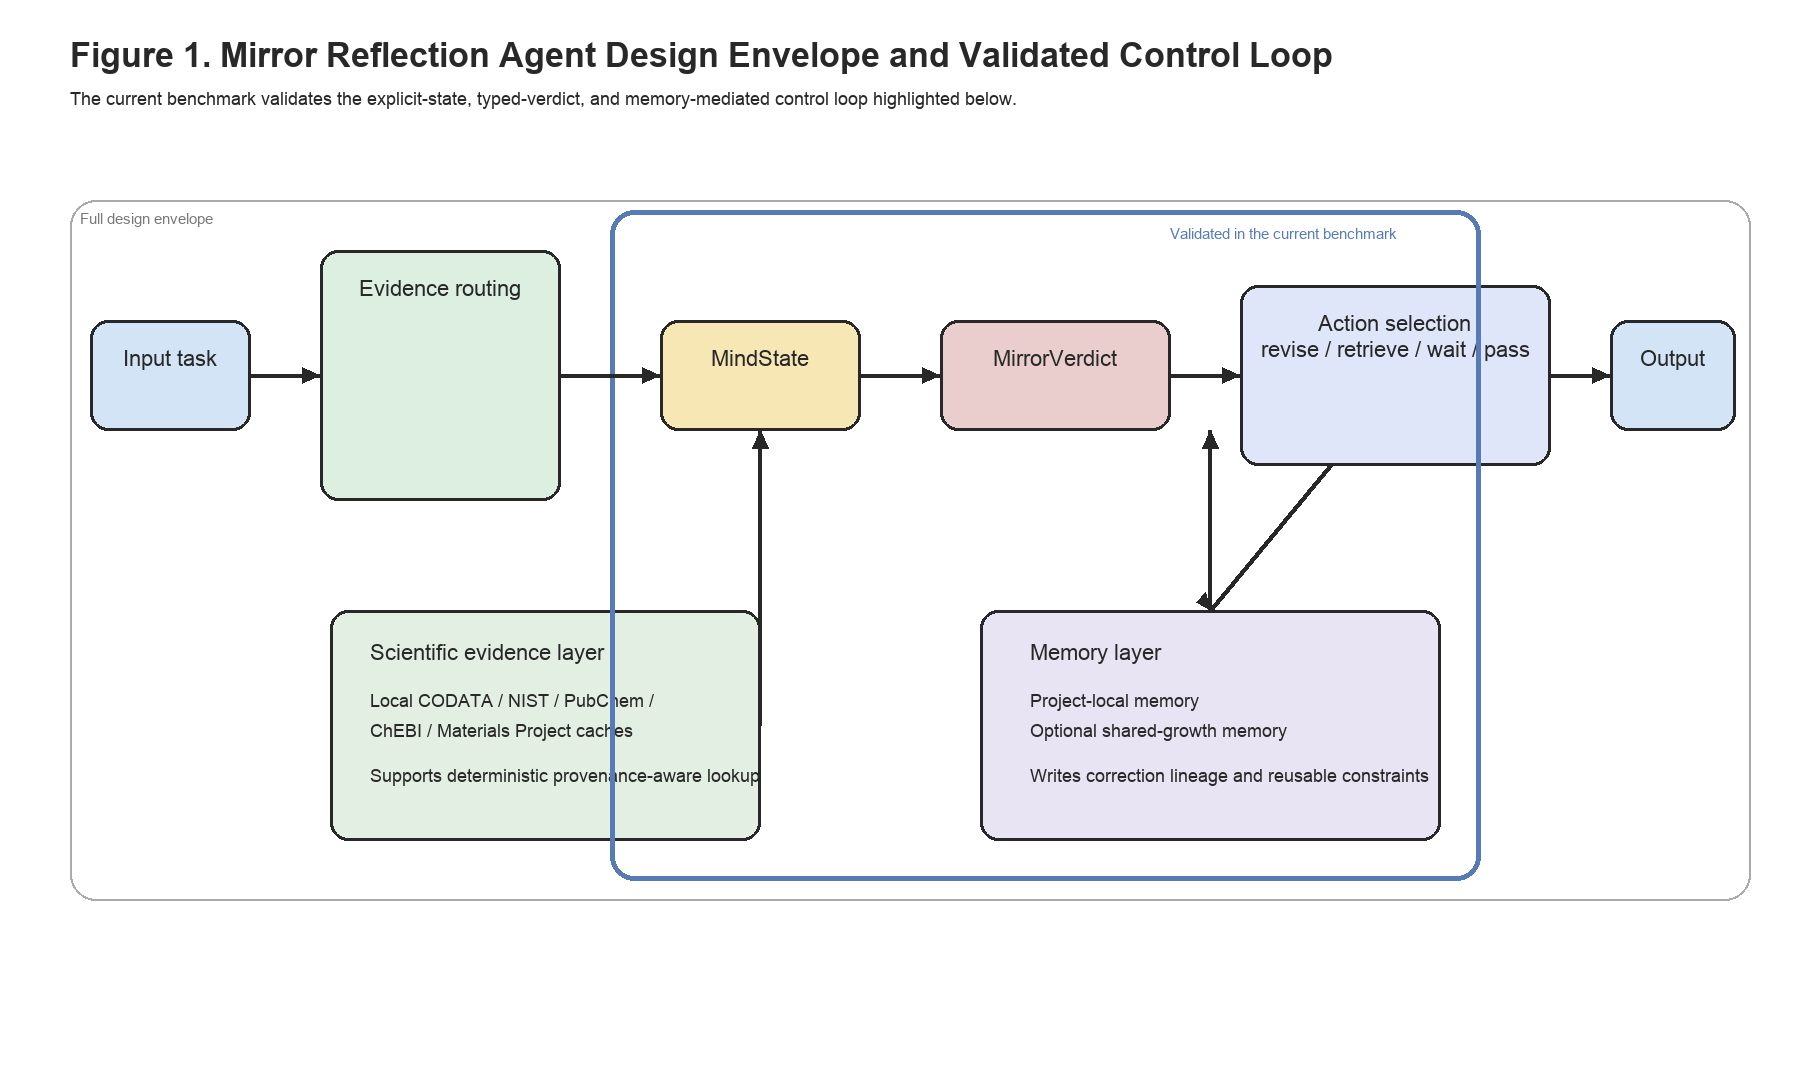
\includegraphics[width=\textwidth]{Figure 1.png}
\caption{Design envelope of Mirror Reflection Agent. The highlighted region corresponds to the explicit-state, typed-verdict, and memory-mediated control loop exercised in the present benchmark, whereas broader evidence routing and deployment coverage remain outside the validated subset.}
\label{fig:v6-architecture}
\end{figure}

Figure~\ref{fig:v6-architecture} separates the overall design envelope from the subset validated in the current study. The benchmark directly exercises the explicit-state, typed-verdict, and memory-mediated control loop, together with locally grounded scientific evidence routing. Broader mixed-problem routing and larger scientific source coverage remain outside the current validation set and should therefore be read as architectural envelope rather than demonstrated capability.

\begin{table}[H]
\centering
\resizebox{\textwidth}{!}{%
\begin{tabular}{lccccc}
\toprule
Method family & Externalized state & Typed verdicts & Correction lineage & Abstention governance & Science-facing condition handling \\
\midrule
Self-Refine & limited & no & no & no & limited \\
Reflexion & partial & no & partial & limited & no \\
CRITIC & partial & no & no & limited & tool-dependent \\
Self-RAG & partial & partial & no & limited & retrieval-aware only \\
Mirror Reflection Agent & explicit & yes & yes & yes & yes, within the current local data envelope \\
\bottomrule
\end{tabular}
}
\caption{Positioning of Mirror Reflection Agent against closely related reflective pipelines. The intended contribution is the combined use of explicit state externalization, typed control verdicts, persistent correction lineage, abstention governance, and science-facing condition handling.}
\label{tab:v6-novelty}
\end{table}

The comparison in Table~\ref{tab:v6-novelty} clarifies the intended novelty. The present work is not simply a claim of ``more reflection''. It combines explicit state objects, typed control actions, persistent correction-lineage memory, and science-facing evidence constraints inside a single inspectable loop. The paper therefore argues for a difference in control structure, not only in prompting style, and is closer in spirit to work on explicit metacognitive control than to prompt-only self-improvement \cite{sofai,academicresponse}.

\subsection{Ablation results}

The clearest evidence for the architecture comes from the ablation study. This track contains 30 cases spanning six reliability families and five scientific themes, each executed under five configurations ranging from direct answering to the full dual-memory loop. The results show that explicit state alone is not enough. The largest gain appears when typed mirror control is introduced, and memory adds a smaller but still meaningful improvement on correction-sensitive families.

\begin{table}[H]
\centering
\resizebox{\textwidth}{!}{%
\begin{tabular}{lcccccccc}
\toprule
Mode & Cases & Pass & Rev. succ. & Condition preserve & Corr. retain & Unsup. cert. & Project-local & Avg. conf. \\
\midrule
Direct answer & 30 & 0.17 & 0.00 & 0.00 & 0.00 & 0.03 & 0.00 & 0.88 \\
MindState only & 30 & 0.33 & 0.00 & 0.67 & 0.00 & 0.03 & 0.00 & 0.82 \\
MindState + Mirror & 30 & 0.57 & 0.33 & 0.67 & 0.00 & 0.03 & 0.00 & 0.58 \\
Mirror + local memory & 30 & 0.70 & 0.43 & 0.60 & 0.13 & 0.03 & 0.13 & 0.57 \\
Mirror + dual memory & 30 & 0.70 & 0.43 & 0.60 & 0.13 & 0.03 & 0.13 & 0.57 \\
\bottomrule
\end{tabular}
}
\caption{Five-way ablation aggregate over 30 cases. ``Rev. succ.'' denotes revision success rate and ``Unsup. cert.'' denotes unsupported-certainty rate.}
\label{tab:v6-track-a-aggregate}
\end{table}

\begin{figure}[H]
\centering
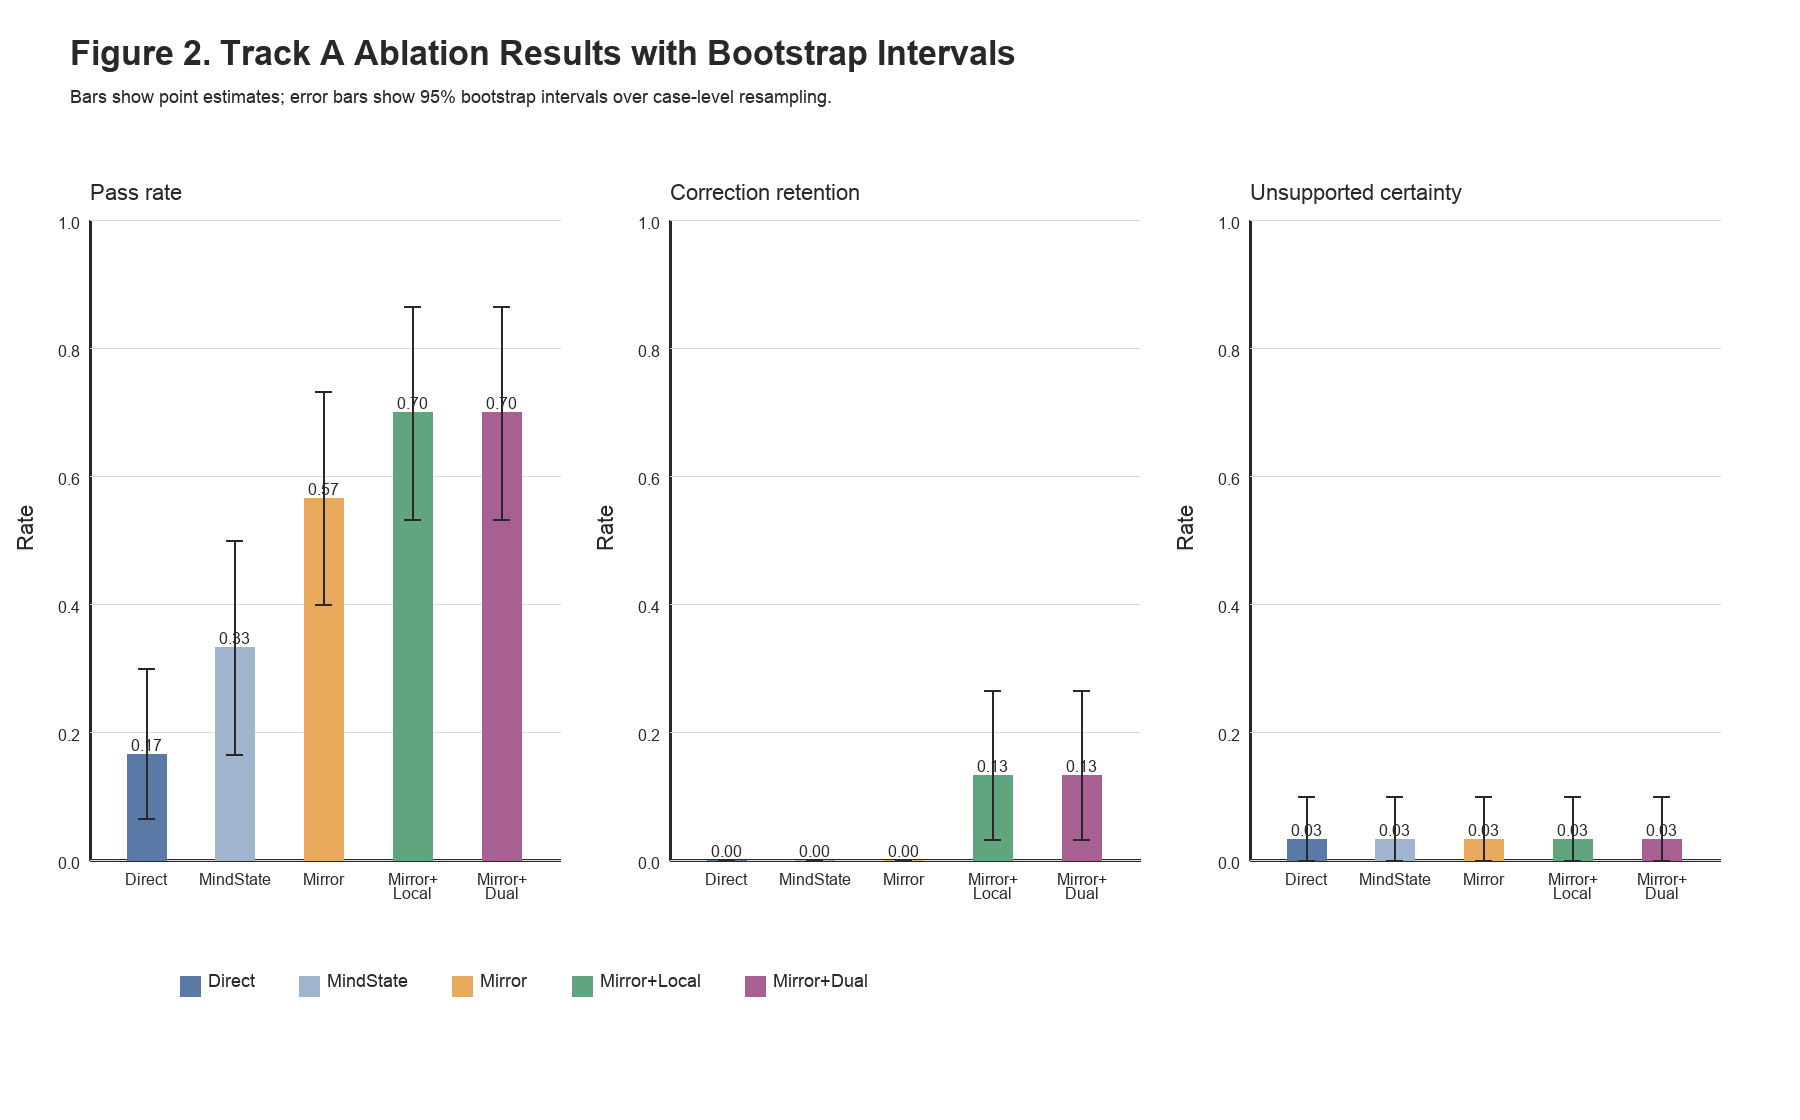
\includegraphics[width=\textwidth]{../results/figures/figure2_ablation.png}
\caption{Ablation summary for Track A. The largest gain appears when typed mirror control is introduced, while memory adds smaller but targeted improvements on correction-sensitive families.}
\label{fig:v6-track-a}
\end{figure}

The aggregate pattern remains consistent after resampling. Pass rate rises from 0.17 in the direct-answer baseline to 0.33 with structured cognition alone and 0.57 once typed mirror control is introduced. Memory-backed modes then reach 0.70, but the aggregate no longer improves when dual memory is added on top of local memory. That pattern matters: most of the gain comes from explicit state plus typed critique, while memory provides targeted benefits on project-local precedence and correction-sensitive cases rather than a uniform lift across all families. Condition preservation increases sharply once the system leaves the direct baseline, and correction retention appears only in memory-backed modes. Bootstrap intervals remain separated between the direct baseline, mirror-only mode, and memory-backed modes, suggesting that the observed gain is associated with control structure rather than with intermediate text alone.

\begin{table}[H]
\centering
\resizebox{\textwidth}{!}{%
\begin{tabular}{lccc}
\toprule
Mode & Pass rate [95\% CI] & Correction retention [95\% CI] & Unsupported certainty [95\% CI] \\
\midrule
Direct answer & 0.17 [0.07, 0.30] & 0.00 [0.00, 0.00] & 0.03 [0.00, 0.10] \\
MindState only & 0.33 [0.17, 0.50] & 0.00 [0.00, 0.00] & 0.03 [0.00, 0.10] \\
MindState + Mirror & 0.57 [0.40, 0.73] & 0.00 [0.00, 0.00] & 0.03 [0.00, 0.10] \\
Mirror + local memory & 0.70 [0.53, 0.87] & 0.13 [0.03, 0.27] & 0.03 [0.00, 0.10] \\
Mirror + dual memory & 0.70 [0.53, 0.87] & 0.13 [0.03, 0.27] & 0.03 [0.00, 0.10] \\
\bottomrule
\end{tabular}
}
\caption{Bootstrap intervals for the primary Track A metrics. Intervals are computed by case-level resampling within each execution mode.}
\label{tab:v6-track-a-uncertainty}
\end{table}

\begin{table}[H]
\centering
\resizebox{\textwidth}{!}{%
\begin{tabular}{lccccc}
\toprule
Track A family & Direct & MindState only & Mirror & Mirror + local & Mirror + dual \\
\midrule
Bounded non-degradation & 1.00 & 1.00 & 1.00 & 1.00 & 1.00 \\
Condition drop & 0.00 & 1.00 & 1.00 & 1.00 & 1.00 \\
Correction reuse & 0.00 & 0.00 & 0.00 & 0.00 & 0.00 \\
Evidence mismatch & 0.00 & 0.00 & 0.80 & 0.80 & 0.80 \\
Project-local precedence & 0.00 & 0.00 & 0.00 & 0.80 & 0.80 \\
Unsupported certainty & 0.00 & 0.00 & 0.60 & 0.60 & 0.60 \\
\bottomrule
\end{tabular}
}
\caption{Family-level pass rates in the ablation benchmark. Each family contains five theme variants.}
\label{tab:v6-track-a-families}
\end{table}

Table~\ref{tab:v6-track-a-families} shows that the architecture is strongest on condition-drop control, evidence-mismatch handling, and project-local precedence. It is weaker on correction reuse, where the current memory path does not yet convert stored lessons into consistent passes, and on unsupported-certainty cases, where mirror control helps but does not eliminate failure. Family-level variability is summarized separately in Fig.~\ref{fig:v6-track-a-heatmap}, which shows that gains are concentrated in governance-heavy families rather than being evenly distributed across the benchmark.

\subsection{Science-facing benchmark results}

The second benchmark grounds the manuscript in deterministic scientific question answering. It contains 36 cases divided across constants-and-units questions, condition-sensitive property questions, and abstention-boundary questions. Ground truth is drawn from local CODATA, NIST WebBook, PubChem/ChEBI, and Materials Project caches \cite{codata2018,nistwebbook,pubchem2023,chebi2013,materialsproject}. Scoring is performed by deterministic extraction and rule checks rather than by an LLM judge, so the benchmark is tightly tied to local structured evidence.

\begin{table}[H]
\centering
\resizebox{\textwidth}{!}{%
\begin{tabular}{llccccc}
\toprule
Category & Mode & Pass & Numeric & Unit & Condition & Abstention \\
\midrule
\multirow{3}{*}{Constants and units}
& Direct answer & 0.000 & 0.917 & 0.917 & 0.000 & 0.000 \\
& Mirror + local & 0.917 & 0.917 & 0.917 & 0.333 & 0.083 \\
& Mirror + dual & 0.917 & 0.917 & 0.917 & 0.333 & 0.083 \\
\midrule
\multirow{3}{*}{Condition-sensitive properties}
& Direct answer & 0.000 & 1.000 & 1.000 & 0.000 & 0.000 \\
& Mirror + local & 0.333 & 0.333 & 0.833 & 0.333 & 1.000 \\
& Mirror + dual & 0.333 & 0.333 & 0.833 & 0.417 & 1.000 \\
\midrule
\multirow{3}{*}{Abstention-boundary cases}
& Direct answer & 0.000 & 1.000 & 1.000 & 0.083 & 0.000 \\
& Mirror + local & 1.000 & 1.000 & 1.000 & 0.500 & 1.000 \\
& Mirror + dual & 1.000 & 1.000 & 1.000 & 0.500 & 1.000 \\
\bottomrule
\end{tabular}
}
\caption{Aggregate results for the science-facing benchmark. ``Numeric'' and ``Unit'' denote numeric accuracy and unit consistency; ``Condition'' denotes condition preservation; ``Abstention'' denotes abstention precision or qualified-answer precision.}
\label{tab:v6-track-b-aggregate}
\end{table}

\begin{figure}[H]
\centering
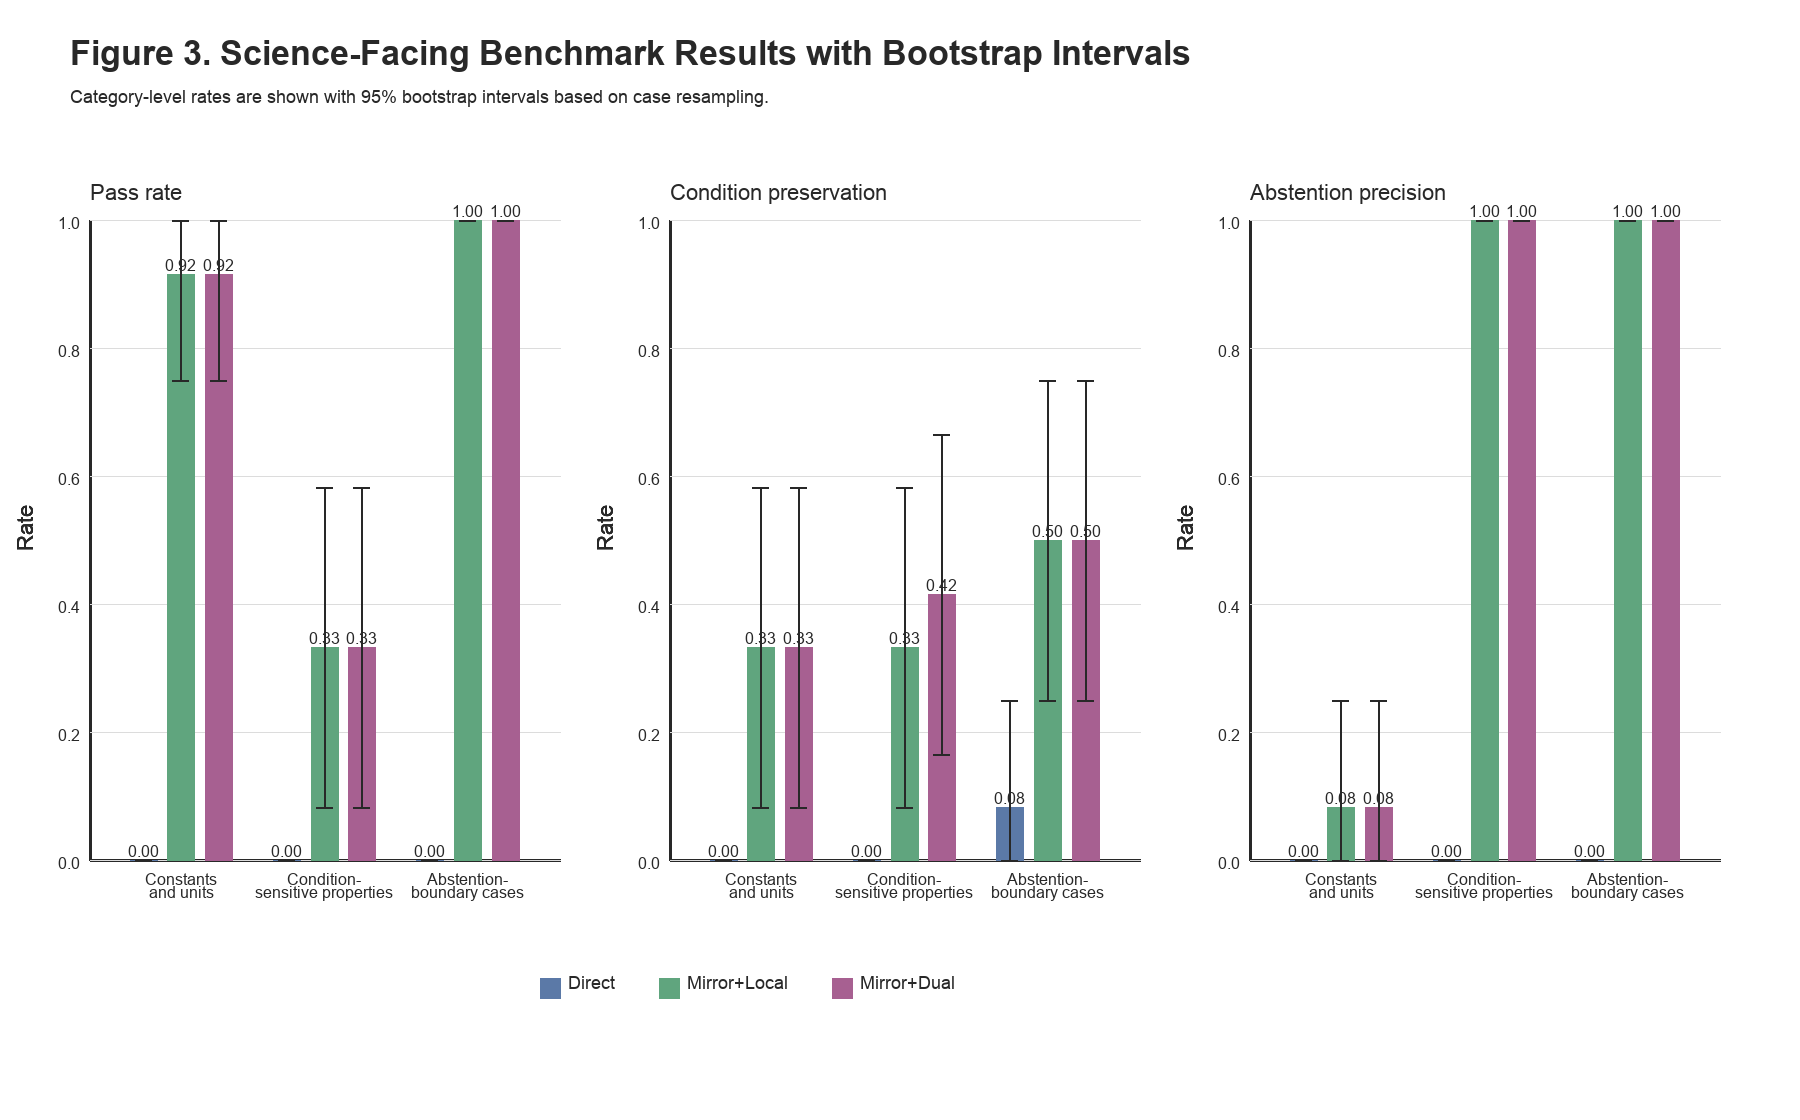
\includegraphics[width=\textwidth]{../results/figures/figure3_science_qa.png}
\caption{Science-facing benchmark results with bootstrap intervals. The direct baseline remains numerically aggressive but weak on provenance, condition handling, and abstention governance.}
\label{fig:v6-track-b}
\end{figure}

Several patterns matter here. On constants-and-units cases, the direct baseline often retrieves the correct number but still fails the category because it omits provenance and condition cues altogether. Reflective modes preserve evidence citation perfectly while matching the same 0.917 numeric accuracy as the direct baseline, which lifts category pass rate to 0.917. On abstention-boundary cases, the direct baseline hallucinates across the full set and scores 0.000 on abstention precision, whereas both reflective memory modes reach 1.000. Within the current local data envelope, these results show a science-facing gain in governance rather than raw lookup alone: the reflective system is substantially more willing to qualify or defer when the cache lacks an exact record or when the requested condition lies outside the supported scope.

The condition-sensitive subset is more mixed and should be read as a central limitation of the current system. The direct baseline attains 1.000 raw numeric accuracy because it emits the first available local record, but it preserves source conditions in none of the cases and therefore scores 0.000 at the category level. Reflective modes improve condition preservation to 0.333 in local-memory mode and 0.417 in dual-memory mode, yet they often defer instead of committing to a conditioned answer. That yields a category-level pass rate of 0.333, with a bootstrap interval of [0.083, 0.583] in both reflective modes. Within the current benchmark, this pattern indicates a coverage--calibration tradeoff with a specific failure point: the mirror policy can detect that a requested answer depends on narrow physical conditions, but the current system still lacks a calibrated path from ``condition recognized'' to ``conditioned answer produced''. The present system is therefore stronger at refusing unsupported extrapolation than at delivering high-yield conditional scientific assistance.

\begin{table}[H]
\centering
\resizebox{\textwidth}{!}{%
\begin{tabular}{llccc}
\toprule
Category & Mode & Pass rate [95\% CI] & Condition preservation [95\% CI] & Abstention precision [95\% CI] \\
\midrule
Constants and units & Direct answer & 0.00 [0.00, 0.00] & 0.00 [0.00, 0.00] & 0.00 [0.00, 0.00] \\
Constants and units & Mirror + local & 0.92 [0.75, 1.00] & 0.33 [0.08, 0.58] & 0.08 [0.00, 0.25] \\
Constants and units & Mirror + dual & 0.92 [0.75, 1.00] & 0.33 [0.08, 0.58] & 0.08 [0.00, 0.25] \\
Condition-sensitive properties & Direct answer & 0.00 [0.00, 0.00] & 0.00 [0.00, 0.00] & 0.00 [0.00, 0.00] \\
Condition-sensitive properties & Mirror + local & 0.33 [0.08, 0.58] & 0.33 [0.08, 0.58] & 1.00 [1.00, 1.00] \\
Condition-sensitive properties & Mirror + dual & 0.33 [0.08, 0.58] & 0.42 [0.17, 0.67] & 1.00 [1.00, 1.00] \\
Abstention-boundary cases & Direct answer & 0.00 [0.00, 0.00] & 0.08 [0.00, 0.25] & 0.00 [0.00, 0.00] \\
Abstention-boundary cases & Mirror + local & 1.00 [1.00, 1.00] & 0.50 [0.25, 0.75] & 1.00 [1.00, 1.00] \\
Abstention-boundary cases & Mirror + dual & 1.00 [1.00, 1.00] & 0.50 [0.25, 0.75] & 1.00 [1.00, 1.00] \\
\bottomrule
\end{tabular}
}
\caption{Bootstrap intervals for the primary Track B metrics. Intervals are computed by case-level resampling within each category and execution mode.}
\label{tab:v6-track-b-uncertainty}
\end{table}

\begin{table}[H]
\centering
\resizebox{\textwidth}{!}{%
\begin{tabular}{lccccc}
\toprule
Mode & Numeric mismatch & Unit mismatch & Condition drop & Missing source & Hallucinated boundary \\
\midrule
Direct answer & 1 & 1 & 12 & 24 & 12 \\
Mirror + local & 9 & 3 & 8 & 8 & 0 \\
Mirror + dual & 9 & 3 & 7 & 8 & 0 \\
\bottomrule
\end{tabular}
}
\caption{Error taxonomy counts across the science-facing benchmark.}
\label{tab:v6-track-b-errors}
\end{table}

The error taxonomy in Table~\ref{tab:v6-track-b-errors} helps explain why the benchmark still supports the manuscript's main claim. The direct baseline is numerically aggressive, but it drops conditions 12 times, omits source cues 24 times, and hallucinates all 12 abstention-boundary cases. Reflective modes still incur numeric misses on the condition-sensitive subset because they sometimes over-defer, but they eliminate hallucinated boundary behavior and sharply reduce missing-source errors.

The case-level traces make this distinction concrete. In case B3-01, the direct baseline returns the 1 atm boiling point of water for a 2 atm query even though the local evidence pack already contains a condition-mismatch warning. In the same case, the reflective dual-memory mode exits with a deferred answer instead of asserting a fabricated value. Conversely, case B2-01 shows the current calibration gap: the reflective local-memory mode detects that the task is condition-sensitive and repeatedly narrows the claim, but ultimately still defers instead of producing a conditioned answer. These paired cases explain why the direct baseline can appear numerically strong while remaining scientifically unreliable, and why the reflective system currently gains more in governance than in answer yield.

\subsection{Longitudinal correction retention}

The third benchmark evaluates whether correction lineage persists across sessions. It contains 10 two-step sequences spanning concept correction, condition-boundary correction, unit correction, abstention correction, and project-vs-shared conflict. In memory-backed modes, step 2 reuses the same temporary memory store as step 1, allowing later behavior to be evaluated against earlier corrections.

\begin{table}[H]
\centering
\resizebox{\textwidth}{!}{%
\begin{tabular}{lcccc}
\toprule
Mode & Cross-session retention & Error recurrence & Memory-scope isolation & Shared-memory pollution \\
\midrule
Direct answer & 0.00 & 0.20 & 0.00 & 0.00 \\
Mirror + local memory & 0.40 & 0.20 & 0.20 & 0.00 \\
Mirror + dual memory & 0.60 & 0.20 & 0.20 & 0.00 \\
\bottomrule
\end{tabular}
}
\caption{Aggregate outcomes for the longitudinal correction benchmark.}
\label{tab:v6-track-c}
\end{table}

\begin{figure}[H]
\centering
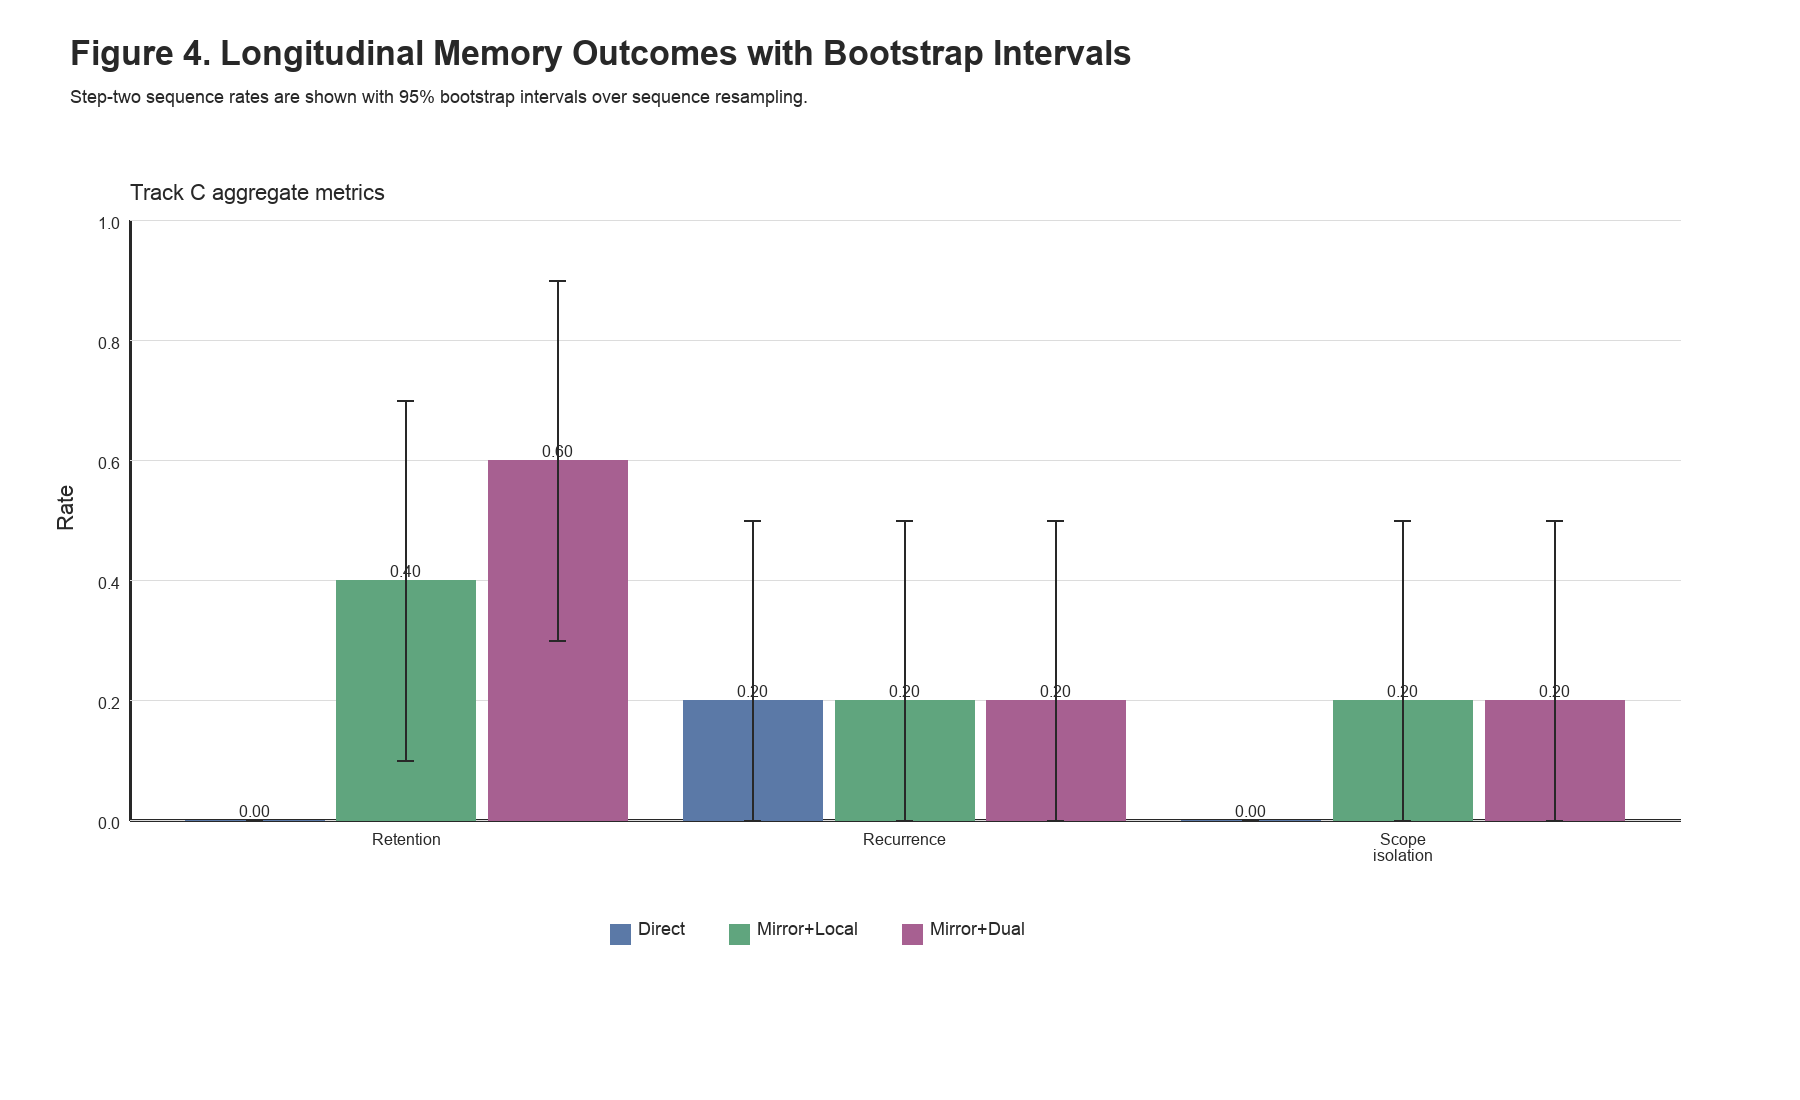
\includegraphics[width=\textwidth]{../results/figures/figure4_longitudinal.png}
\caption{Longitudinal retention results with bootstrap intervals. Reflective memory modes improve correction retention, but recurrence remains unresolved in one sequence family and scope isolation stays weak.}
\label{fig:v6-track-c}
\end{figure}

The longitudinal results are mixed but still informative. Direct answering retains no correction lineage and exhibits a 0.20 recurrence rate. Local memory raises cross-session correction retention to 0.40, and dual memory raises it further to 0.60, but neither configuration eliminates recurrence in the current sequence suite because one abstention-correction family remains unresolved. The corresponding bootstrap interval for dual-memory retention is [0.30, 0.90], which is encouraging but still wide because the benchmark contains only 10 two-step sequences. The shared-memory pollution heuristic remains at 0.00. At the same time, memory-scope isolation remains weak at 0.20, with a bootstrap interval of [0.00, 0.50], which suggests that the current scope policy should not yet be treated as mature.

\begin{table}[H]
\centering
\resizebox{\textwidth}{!}{%
\begin{tabular}{lccc}
\toprule
Mode & Correction retention [95\% CI] & Error recurrence [95\% CI] & Scope isolation [95\% CI] \\
\midrule
Direct answer & 0.00 [0.00, 0.00] & 0.20 [0.00, 0.50] & 0.00 [0.00, 0.00] \\
Mirror + local memory & 0.40 [0.10, 0.70] & 0.20 [0.00, 0.50] & 0.20 [0.00, 0.50] \\
Mirror + dual memory & 0.60 [0.30, 0.90] & 0.20 [0.00, 0.50] & 0.20 [0.00, 0.50] \\
\bottomrule
\end{tabular}
}
\caption{Bootstrap intervals for the primary Track C metrics. Intervals are computed over the step-two sequence cases only.}
\label{tab:v6-track-c-uncertainty}
\end{table}

The sequence-level traces clarify what these aggregates mean. In case C-Seq03-S2, the reflective dual-memory mode retrieves the earlier correction about unsupported pressure conditions and waits instead of extrapolating from the 1 atm record. This is the intended use of correction lineage. At the same time, the abstention-correction family shows that a stored lesson does not automatically translate into a passing outcome: the system can still defer without turning that abstention into a more stable correction policy. The current benchmark therefore remains a controlled two-step setting, and its sequence length is too short to support stronger claims about long-horizon memory behavior.

\subsection{Reproducibility}

The redesigned benchmark produces a complete artifact tree under \texttt{results/}, including raw JSON outputs for every run, per-track aggregate summaries, CSV tables, and manuscript-ready figures. In total, the benchmark executes 318 runs from 86 unique cases: 150 runs for the ablation benchmark, 108 runs for the science-facing benchmark, and 60 runs for the longitudinal benchmark. These assets make the current study substantially easier to inspect and replay than earlier drafts built around a minimal proof-of-mechanism suite.

\begin{figure}[H]
\centering
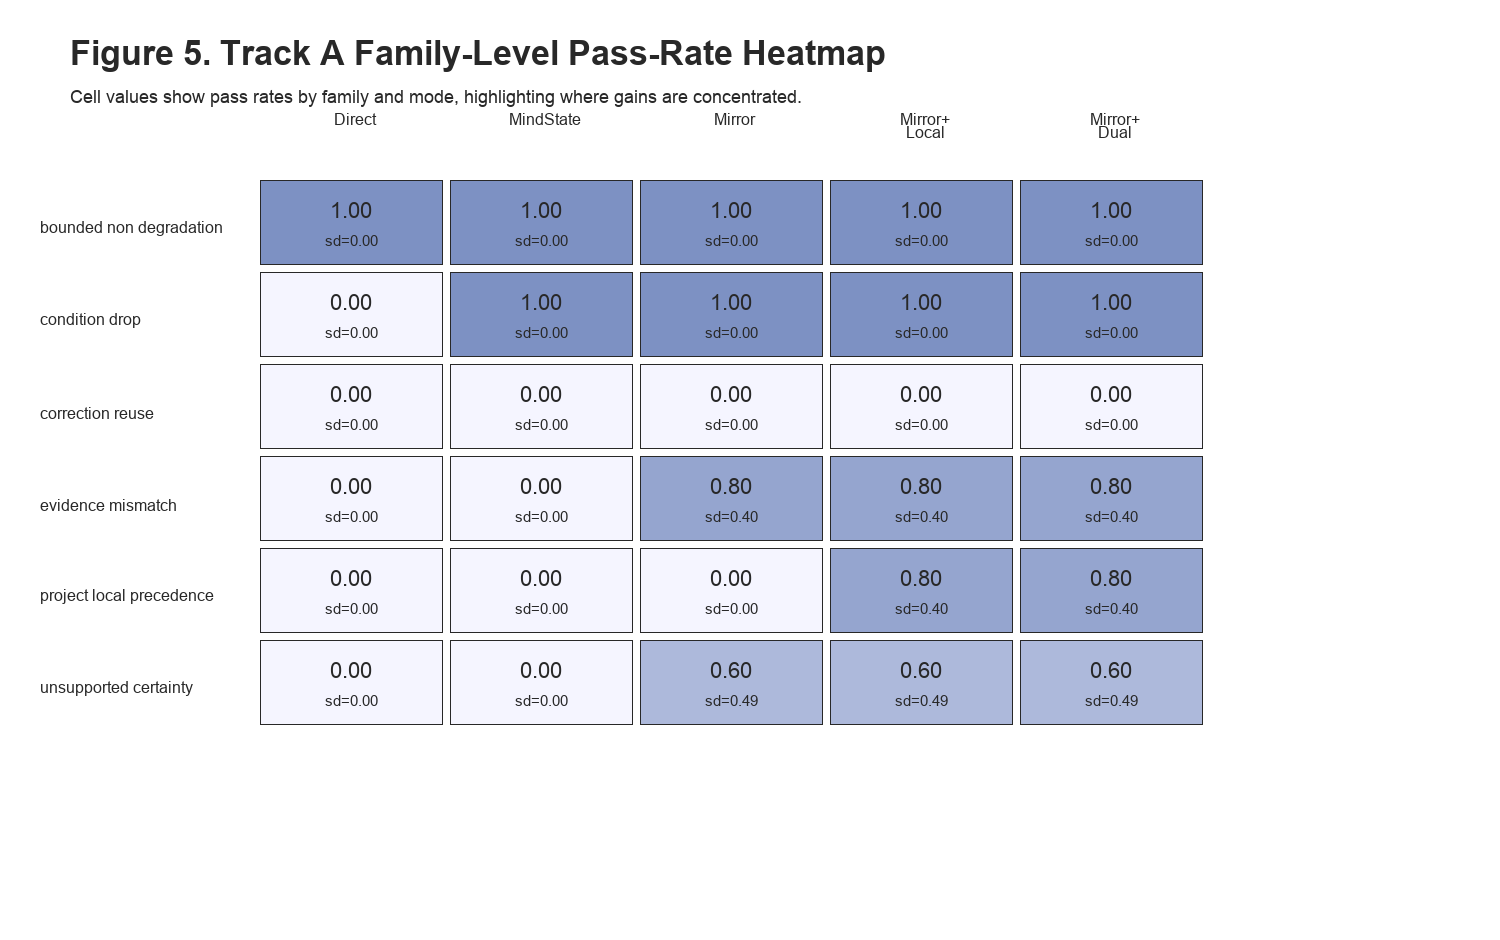
\includegraphics[width=\textwidth]{../results/figures/figure5_track_a_heatmap.png}
\caption{Family-level pass-rate heatmap for Track A. Gains are concentrated in condition-drop control, evidence-mismatch handling, and project-local precedence, while correction reuse remains unresolved in the current implementation.}
\label{fig:v6-track-a-heatmap}
\end{figure}

\section{Discussion}

Taken together, the current results support Mirror Reflection Agent as a science-facing systems and mechanism contribution. The strongest evidence is architectural and behavioral: explicit state, typed mirror critique, and correction-lineage memory measurably change what the system does. The ablation study shows that these gains are not reducible to prompt length alone. The science-facing benchmark shows that the same control structure can improve evidence citation and abstention behavior on deterministic scientific tasks. The longitudinal benchmark shows that correction lineage can influence later behavior without measured shared-memory pollution in the current suite.

The results also clarify where this architecture differs from reflection systems aimed at general academic writing. In those settings, stored reflections function mainly as rhetorical or strategic guidance for producing better responses. Here, the value of memory lies in recording factual boundaries, failure modes, and correction lineage that should constrain later scientific claims. That distinction matters most in local or privacy-sensitive settings, where the system must remain traceable to local evidence sources and where unsupported extrapolation can be more damaging than stylistic weakness.

The present limitations remain substantial. The scientific data envelope is narrow because it is restricted to local CODATA, NIST WebBook, PubChem/ChEBI, and Materials Project caches bundled with the repository. The direct baseline is intentionally naive and should be interpreted as an architecture-first reference rather than as a strong scientific agent baseline. The condition-sensitive family reveals conservative over-deferral: the current mirror policy often treats narrow-condition warnings as reasons to keep revising or to defer, even when a more calibrated conditioned answer might be acceptable. In addition, memory-scope isolation remains weak in the longitudinal benchmark, and one sequence family still exhibits recurrence under all modes, which keeps the current memory evidence clearly bounded.

These limits define the boundary of the paper. The manuscript does not establish broad scientific superiority, general continual learning, or full AI-for-Science coverage. What it does show is that a structured reliability-control architecture can produce auditable, bounded gains on science-facing tasks, and that those gains can be measured with a deterministic benchmark rather than with opaque judge prompts. More broadly, the paper suggests that reliability gains need not come only from model scale or from prompt-only self-reflection. They can also emerge from explicit state design, typed control flow, and auditable memory structures, which may be especially valuable in local, resource-constrained, or data-sensitive scientific deployments. Within that boundary, the present benchmark supports the architecture most strongly as a scientific claim-governance mechanism, not as a fully mature scientific answering system.

\section{Methods}

\subsection{System implementation}

Mirror Reflection Agent is organized as four layers. The perception layer receives user input and task descriptions. The cognition layer produces a structured \texttt{MindState} rather than a direct final answer. The mirror layer critiques the candidate state for premature convergence, concept blending, evidence gaps, overclaiming, old-template reuse, and scientific condition or unit problems. The seed-memory layer stores facts, contexts, bias lineage, correction lineage, and reusable strategies in project-local memory, with an optional dual-layer shared-growth backend. The current implementation uses deterministic control logic and replayable audit traces. Scientific evidence is retrieved from local CODATA, NIST WebBook, PubChem/ChEBI, and Materials Project caches \cite{codata2018,nistwebbook,pubchem2023,chebi2013,materialsproject}, while commonsense evidence is routed through a separate layer and kept subordinate to structured factual sources.

This implementation choice is deliberate. The benchmark is designed for local auditability rather than for maximum open-ended coverage. Memory therefore records correction lineage and reusable boundary lessons tied to local evidence, not rhetorical templates for producing more persuasive text. The same design also makes the current system suitable for scientific settings in which unpublished data, local traceability, or deployment constraints make cloud-dependent judge loops undesirable.

\subsection{Validated scope}

\begin{table}[H]
\centering
\resizebox{\textwidth}{!}{%
\begin{tabular}{lcccc}
\toprule
Component & Implemented in code & Exercised in benchmark & Used in main claim & Deferred to future work \\
\midrule
MindState generation & yes & yes & yes & no \\
Mirror verdict logic & yes & yes & yes & no \\
Project-local memory & yes & yes & yes & no \\
Dual/shared memory & yes & yes & yes & no \\
Scientific evidence routing & yes & yes, within local sources & yes & broader source coverage \\
Commonsense routing & yes & yes, mainly in internal reliability cases & supporting only & broader mixed-problem evaluation \\
Mixed-problem path & partially & no & no & yes \\
External data source envelope & partially & no, beyond local bundled caches & no & yes \\
\bottomrule
\end{tabular}
}
\caption{Implemented, exercised, and deferred scope. The table separates the full system envelope from the subset actually validated by the present benchmark.}
\label{tab:v6-scope}
\end{table}

Table~\ref{tab:v6-scope} makes the claim boundary explicit. The benchmark validates the control loop, mirror logic, memory behavior, and science-facing use of the local data envelope. It does not validate large-scale external scientific benchmarking or the full mixed-problem routing envelope suggested by the overall architecture.

\subsection{Benchmark construction}

The evaluation uses a unified case schema that records case identifier, track, family, ablation level, prompt, goal, injected error or risk target, required execution modes, project-local and shared seed memories, ground truth, source information, expected verdict sequence, expected revision count, pass rules, fail rules, metrics under test, notes, and, for the longitudinal benchmark, sequence identifier and sequence step. In addition, the schema preserves whether a case is serving as an ablation, a science-facing query, or a longitudinal correction sequence. Each executed run is written as a raw JSON file containing the case payload, selected seeds, final state, verdict, trace, extracted scoring fields, and rule-evaluation results.

The ablation benchmark contains 30 cases built from six reliability families and five scientific themes. The science-facing benchmark contains 36 deterministic scientific cases divided across constants-and-units questions, condition-sensitive property questions, and abstention-boundary questions. The longitudinal benchmark contains 10 two-step sequences covering concept correction carryover, condition-boundary correction, unit correction, abstention correction, and project-vs-shared conflict. For memory-backed modes in the longitudinal benchmark, step two reuses the same temporary memory store as step one so that correction carryover can be measured directly.

\begin{table}[H]
\centering
\resizebox{\textwidth}{!}{%
\begin{tabular}{lccccc}
\toprule
Track & Cases & Modes & Runs & Primary metrics & Scientific purpose \\
\midrule
A & 30 & 5 & 150 & Pass rate; correction retention; unsupported certainty & Isolate control-structure gains \\
B & 36 & 3 & 108 & Pass rate; condition preservation; abstention precision & Test evidence-bounded scientific behavior \\
C & 20 & 3 & 60 & Retention; recurrence; scope isolation & Test cross-session correction carryover \\
\bottomrule
\end{tabular}
}
\caption{Overview of the benchmark design used in the manuscript.}
\label{tab:v6-overview}
\end{table}

\subsection{Execution modes}

Five execution modes are used across the benchmark. The direct-answer mode emits a naive direct claim from the first available evidence without mirror governance. The mind-state-only mode produces a structured cognitive state but does not invoke the mirror. The mirror-only mode runs cognition and mirror without memory. The local-memory mode runs the full reflective loop with project-local memory. The dual-memory mode runs the full reflective loop with project-local and shared-growth memory. Not every track uses every mode: the full five-way suite appears only in Track A, while Tracks B and C compare the direct baseline against the two memory-backed reflective configurations.

\subsection{Metric rubric}

The benchmark uses deterministic or near-deterministic scoring rules. Pass rate measures the fraction of cases that satisfy the structured pass rules attached to each case. Revision success rate measures the fraction of cases that revise at least once and still satisfy those rules. Premature-convergence rate and concept-mixing rate measure whether the final claim still triggers the corresponding mirror detectors. Correction-retention rate measures whether designated step-two cases preserve the expected correction fragment in either the output or the retrieved lessons. Unsupported-certainty rate measures whether the output still contains strong certainty markers unsupported by the current evidence. This emphasis on explicit and replayable scoring is intended to complement prior reflection work that is often evaluated with broader generation metrics or human preference judgments \cite{selfrefine,reflexion,critic,academicresponse}. The scoring engine follows a fixed rule-matching priority: verdict checks are applied first, followed by numeric and unit matching, revision-count checks, correction-retention checks, and finally heuristic boundary metrics such as shared-memory pollution risk.

For the science-facing benchmark, numeric accuracy is determined by matching the extracted answer value against the local record with a task-specific tolerance, and unit consistency is determined by matching the extracted unit against the local record. Numeric extraction follows a fixed priority rule that first searches for the value adjacent to the expected unit, then falls back to the first well-formed numeric token in the final claim. Condition preservation records whether the output keeps the relevant condition fragment visible. Evidence citation presence records whether the output mentions one of the expected local source identifiers. Abstention precision records whether a boundary case is deferred or qualified instead of being answered as a fact. Shared-memory pollution risk is computed heuristically from the stored shared-memory records using allowed value types and excluded contamination patterns. Track B ground truth is derived only from local structured caches, and no LLM judge is used at any stage.

\subsection{Uncertainty estimation and robustness analysis}

The main rates reported in the manuscript are accompanied by bootstrap confidence intervals computed from case-level resampling within each track and execution mode. For Track A, resampling is performed across the 30 ablation cases within each mode, and intervals are reported for pass rate, correction retention, and unsupported certainty. For Track B, resampling is performed separately within each category-mode slice over 12 cases per slice, and intervals are reported for pass rate, condition preservation, and abstention precision. For Track C, resampling is performed across the 10 step-two sequence cases for each mode, and intervals are reported for cross-session correction retention, error recurrence, and memory-scope isolation.

Family-level variability is reported separately from aggregate rates. In Track A, each family-mode cell includes both a pass-rate estimate and the standard deviation of case-level outcomes within that family. In Track B, variability is summarized within category-mode slices to expose the spread hidden by aggregate category means. In Track C, family-level retention is reported across the five sequence families. The error categories listed in Table~\ref{tab:v6-track-b-errors} are not mutually exclusive: a single case can contribute simultaneously to numeric mismatch, missing source, and condition-drop counts. This choice is intentional because the error taxonomy is meant to represent failure surfaces rather than a partition of the dataset.

\subsection{Artifact release and reproducibility}

All evidence reported in the manuscript is generated from the repository's local benchmark pipeline. The current run writes raw outputs to \texttt{results/raw/A}, \texttt{results/raw/B}, and \texttt{results/raw/C}, aggregate summaries to \texttt{results/aggregate/*.json}, manuscript tables to \texttt{results/tables/*.csv}, manuscript-ready figures to \texttt{results/figures/*.png}, and a release manifest plus environment snapshot to \texttt{results/release/}. These assets are organized so that the same evidence can be mirrored into an anonymized review package without hidden manual judgments.

\section*{Data availability}

The benchmark cases, aggregate summaries, raw execution outputs, generated CSV tables, figure assets, release manifest, and environment snapshot reported in this manuscript are stored in the project repository under \texttt{results/}. For peer review, an anonymized package can be assembled directly from these assets. Ground-truth scientific records are drawn from local CODATA, NIST WebBook, PubChem/ChEBI, and Materials Project caches bundled with the repository; any non-public cache limitations are documented in \texttt{results/release/release\_manifest.json}.

\section*{Code availability}

The current prototype, the benchmark generator, the robustness-analysis script, and the manuscript sources are maintained in the same local repository used to generate this draft. The intended review package consists of the manuscript sources together with the benchmark runner, raw outputs, figure-generation scripts, and the environment snapshot stored under \texttt{results/release/environment\_snapshot.txt}.

\begin{thebibliography}{16}
\bibitem{cot}
Wei, J. et al. Chain-of-thought prompting elicits reasoning in large language models. arXiv preprint arXiv:2201.11903 (2022).

\bibitem{react}
Yao, S., Zhao, J., Yu, D., Du, N., Shafran, I., Narasimhan, K. \& Cao, Y. ReAct: Synergizing reasoning and acting in language models. In \textit{The Eleventh International Conference on Learning Representations} (2023).

\bibitem{toolformer}
Schick, T. et al. Toolformer: Language models can teach themselves to use tools. arXiv preprint arXiv:2302.04761 (2023).

\bibitem{selfrefine}
Madaan, A. et al. Self-refine: Iterative refinement with self-feedback. arXiv preprint arXiv:2303.17651 (2023).

\bibitem{reflexion}
Shinn, N., Cassano, F., Gopinath, A., Narasimhan, K. \& Yao, S. Reflexion: Language agents with verbal reinforcement learning. In \textit{Advances in Neural Information Processing Systems 36} (2023).

\bibitem{critic}
Gou, Z. et al. CRITIC: Large language models can self-correct with tool-interactive critiquing. In \textit{The Twelfth International Conference on Learning Representations} (2024).

\bibitem{selfrag}
Asai, A. et al. Self-RAG: Learning to retrieve, generate, and critique through self-reflection. In \textit{The Twelfth International Conference on Learning Representations} (2024).

\bibitem{sofai}
Bergamaschi Ganapini, M. et al. Fast, slow, and metacognitive thinking in AI. \textit{npj Artif. Intell.} \textbf{1}, 27 (2025).

\bibitem{academicresponse}
Li, B. \& Zhao, C. Self-reflection enhances large language models towards substantial academic response. \textit{npj Artif. Intell.} \textbf{1}, 45 (2025).

\bibitem{codata2018}
Tiesinga, E., Mohr, P. J., Newell, D. B. \& Taylor, B. N. CODATA recommended values of the fundamental physical constants: 2018. \textit{Rev. Mod. Phys.} \textbf{93}, 025010 (2021).

\bibitem{nistwebbook}
Linstrom, P. J. \& Mallard, W. G. The NIST Chemistry WebBook: A chemical data resource on the Internet. \textit{J. Chem. Eng. Data} \textbf{46}, 1059--1063 (2001).

\bibitem{pubchem2023}
Kim, S. et al. PubChem 2023 update. \textit{Nucleic Acids Res.} \textbf{51}, D1373--D1380 (2023).

\bibitem{chebi2013}
Hastings, J. et al. The ChEBI reference database and ontology for biologically relevant chemistry: Enhancements for 2013. \textit{Nucleic Acids Res.} \textbf{41}, D456--D463 (2013).

\bibitem{materialsproject}
Jain, A. et al. Commentary: The Materials Project: A materials genome approach to accelerating materials innovation. \textit{APL Mater.} \textbf{1}, 011002 (2013).
\end{thebibliography}

\end{document}
